\documentclass{neu_handout}
\usepackage{url}
\usepackage{amssymb}
\usepackage{amsmath}
\usepackage{marvosym}
\usepackage{graphicx}
\usepackage[pdftex]{graphicx}
\usepackage{subfigure}
\usepackage{listings}
\usepackage{color}

\definecolor{dkgreen}{rgb}{0,0.6,0}
\definecolor{gray}{rgb}{0.5,0.5,0.5}
\definecolor{mauve}{rgb}{0.58,0,0.82}

\lstset{frame=tb,
  language=Python,
  aboveskip=3mm,
  belowskip=3mm,
  showstringspaces=false,
  columns=flexible,
  basicstyle={\small\ttfamily},
  numbers=none,
  numberstyle=\tiny\color{gray},
  keywordstyle=\color{blue},
  commentstyle=\color{dkgreen},
  stringstyle=\color{mauve},
  breaklines=true,
  breakatwhitespace=true,
  tabsize=3
}

\graphicspath{ {images/} }
\everymath{\displaystyle}

% Professor/Course information
\title{Classifying High-Resolution Brain Scans using Apache Spark}
\author{Asha Chen-Phang, Emily Dutile, Nate Otenti, Tristan Sweeney}
\date{April 2018}
\course{EECE 5644}{Pattern Recognition and Machine Learning}

\begin{document}

\section*{1 Introduction}
Being in the multi-core and machine learning era, it is important for our machine learning algorithms to take advantage of the potential speed up through the use of paralleling tasks on multi-core computers and distributed systems. With an interest in processing a massive image dataset and using well-known industry solution for faster computation, the group used Apache Spark, a processing model for analyzing big data, to analyze the speed up of machine learning algorithms for foreground-background classification in high-resolution brain scans. With the dataset, we performed preprocessing, feature extraction, implemented Random Forest in python using sklearn in a single-processor solution, and implemented Random Forest in scala on top of Apache Spark using MLlib to analyze time and processing efficiency in a parallel processing program upon distributed data. The Apache Spark environment was created on an Amazon EMR cluster, leveraging the EMR file system (EMRFS) to access data in Amazon S3.\\

We worked with a dataset with the interest of turning high-resolution brain scans, as seen in the left figure \ref{fig:left}, into a graph representing nerve connections indicated by the bright lines. The original image is 3-dimensional. For better intuition the 2-dimensional projection on the X-Y plane is shown. As you can see, the image is noisy but the axons, which are the lines going across the image, are clearly visible. To improve the quality of algorithms that automatically trace these axons in an image, we classified each pixel as foreground (belongs to an axon) or background (does not belong to an axon). The traced data looks like the figure on the right\ref{fig:right}, where white indicates foreground and black indicates background.\\

\begin{figure}[h]
\centering
{
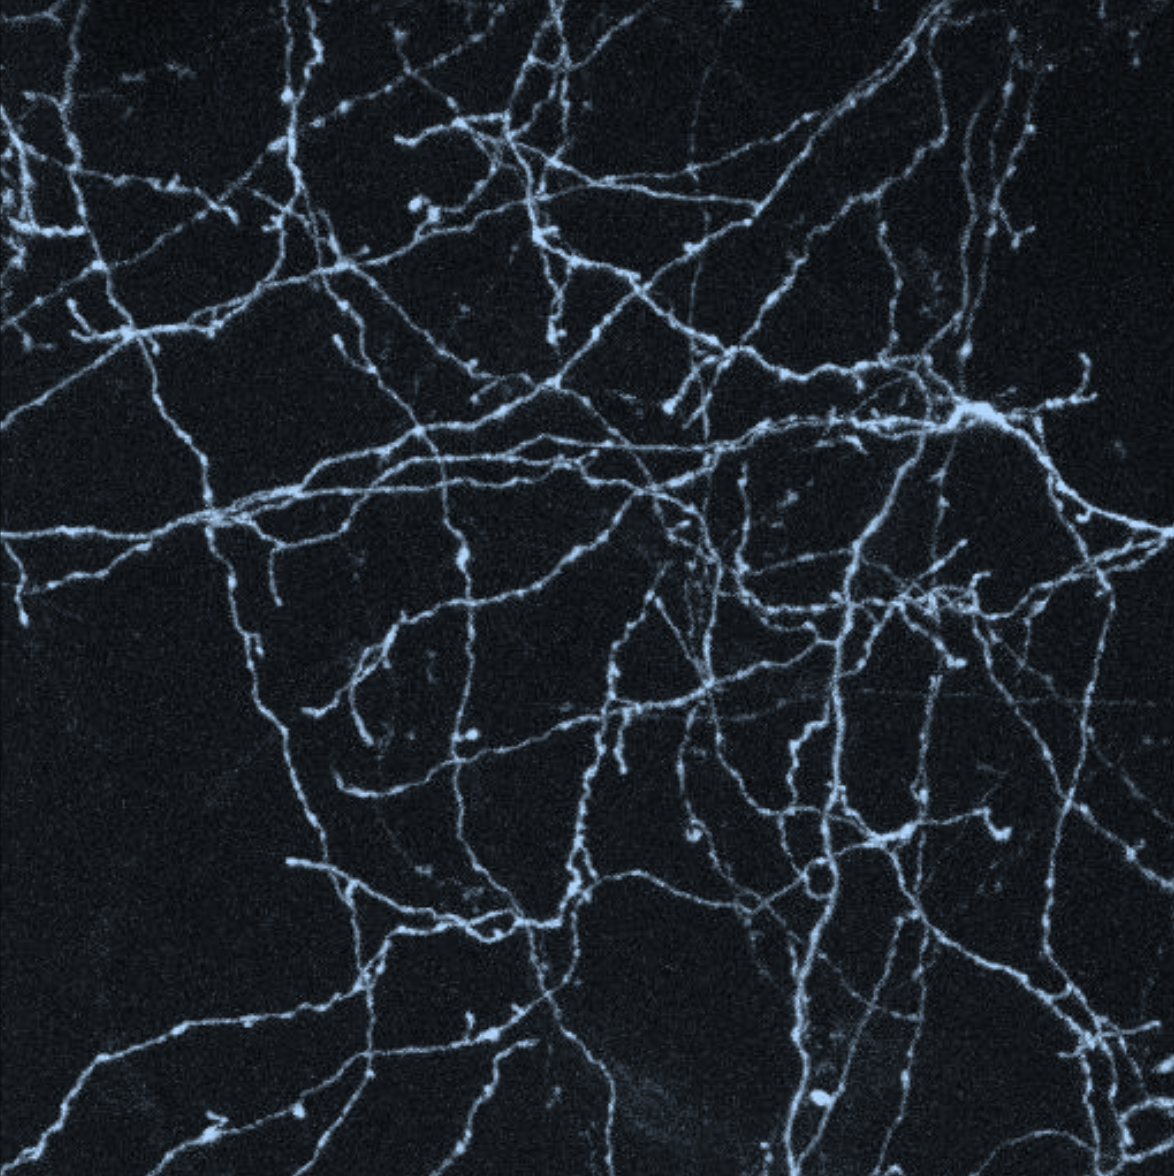
\includegraphics[width=0.2\linewidth]{image1}
\label{fig:left}
}
{
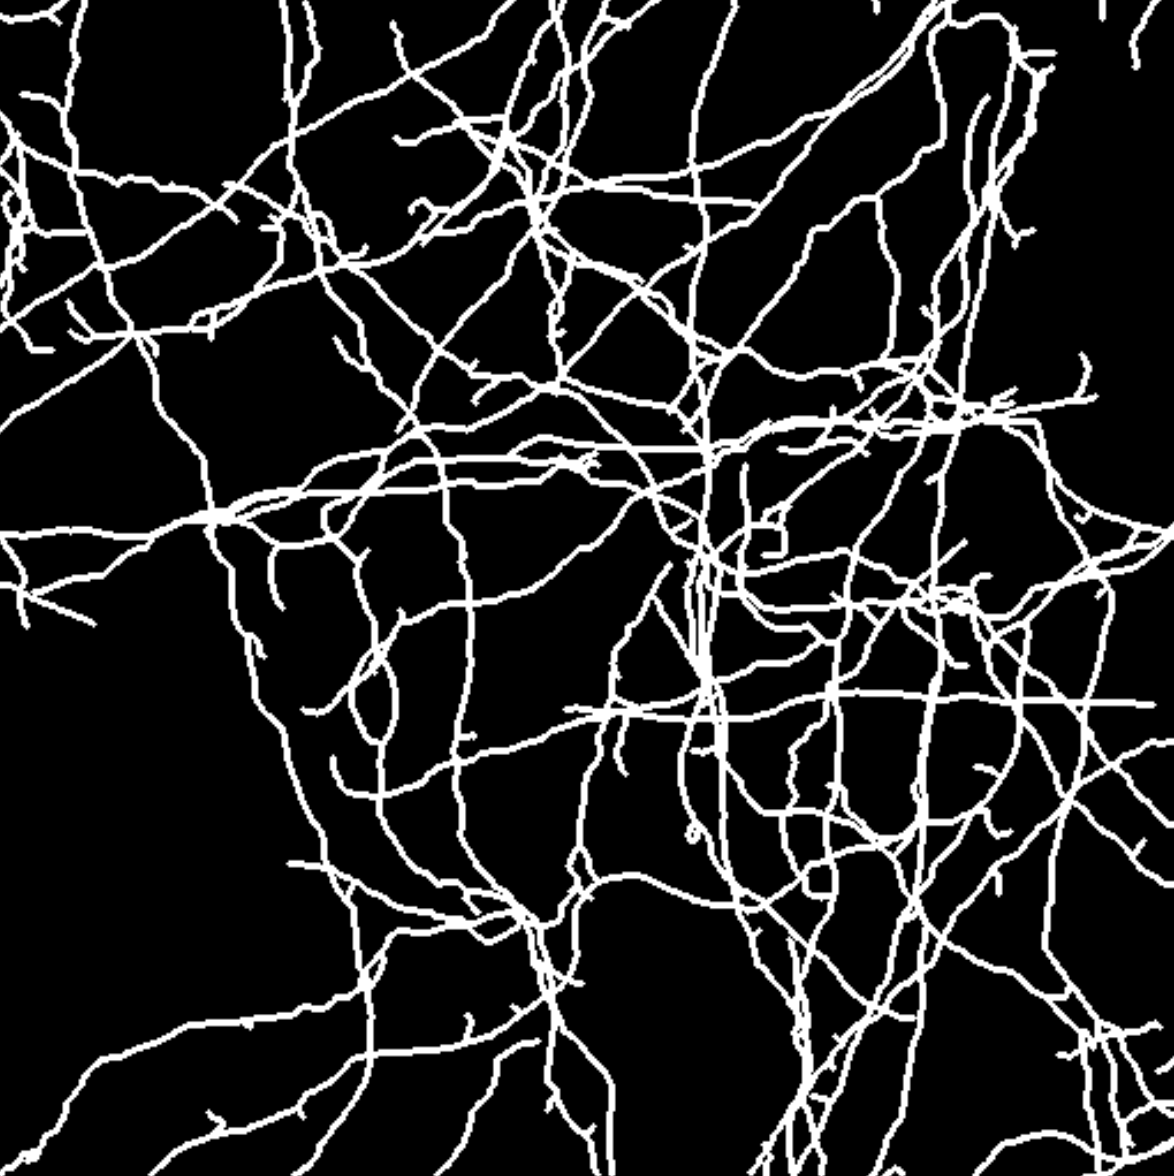
\includegraphics[width=0.2\linewidth]{image2}
\label{fig:right}
}
\end{figure}


Using the manually traced image, the labeled data was generated as follows:
\newenvironment{myitemize}
{ \begin{itemize}
    \setlength{\itemsep}{0pt}
    \setlength{\parskip}{0pt}
    \setlength{\parsep}{0pt}     }
{ \end{itemize}                  } 

\begin{myitemize}
  \item Select a pixel (i, j, k) in the image.
  \item Extract a neighborhood vector centered around (i, j, k).
  \item Extract the label of (i, j, k) from the trace. Here 1 indicates foreground; 0 indicates background.
  \item  Save the record as the neighborhood vector, followed by the label.
\end{myitemize}

Assuming pixel (i=10, j=10, k=10) was selected and we are working with a neighborhood of size 3x3x3, these 27 pixels would be stored as a vector n with 27 elements, where n[0] stores the brightness value of
pixel (9, 9, 9), n[1] the brightness of (9, 9, 10), n[2] of (9, 9, 11), n[3] of (9, 10, 9), n[4] of (9, 10, 10), and so on. Neighborhoods of size 21x21x7 were recommended by domain experts, which is what the labeled data sets contain.\\

\subsection*{1.1 The Data}
The dataset\footnote{\url{https://drive.google.com/drive/u/0/folders/1EJBgJFmp-FQf2czw9LGImoOhEO2OvOoo}} is composed of several labeled csv files, each consisting of rows that contain an input vector of 21x21x7
brightness values (intensity) from a 3D image, together with the center pixel's foreground-vs-background label. The last value is the label for the whole image. On each line there are 21*21*7+1 values. Each image, which is a csv file, is roughly 6.5 GB. The labeled data from images 1, 2, 3, 4, and 6 are used to train the most accurate model for predicting the labels in image 5 of the datasets. In the final evaluation set, there are nearly 0.0057\% foreground and 99.99\% background pixel. For classification accuracy, a high value does not necessarily mean the model is performing well. In our case, the "dumb" model that always predicts label 0 for every input will have 99\% accuracy, so any model achieving less than 99\% would not be beating the dumb model. \\

Using the standard way of training and testing a classification model, the labeled data is partitioned into 3 separate sets: training, validation and test data. Uniform random partitioning into training and validation data often works well, but there are datasets, such as this one, where it is not sufficient. Assume we have two labeled records with centers (x,y,z) and (x+1, y+1, and z+1). Uniform sampling could assign (x,y,z) to training and (x+1, y+1, and z+1) to the validation data. The two neighborhoods and labels of the two pixels are highly correlated. The model would overfit to the training data and give overly optimistic validation accuracy from the correlations. To ensure independent training and validation, partitioning by image is needed.\\

\section*{2 Related Works}

\section*{3 Methods}
Various models were evaluated in order to receive the highest accuracy of predictions on the high resolution brain scans\footnote{\url{https://drive.google.com/drive/u/0/folders/1EJBgJFmp-FQf2czw9LGImoOhEO2OvOoo}} such as Linear SVM, Nearest Neighbor, Decision Tree, Neural Net and AdaBoost. The model that gave us the best results was Random Forest. Random forests is a well-known ensemble method that's used to build predictive classification models. The model creates an entire forest of random uncorrelated decision trees to arrive at the best possible answer. Random Forest looks to reduce a correlation issue, a limitation to bagging trees, through choosing a subsample of the feature space at each split by using a stopping criteria for node splits to prune the trees. Exploration of multiple parameter combinations was explored to achieve the best possible accuracy. \\

To begin visualizing the data, we performed our analysis using Jupyter Notebooks, numpy, and matplotlib. To do so, we took one of the csv files, found the rows of the file that are labeled as 1, found the rows of the file that has 0 as the label, and generated a file with 100 "foreground" images and 100 "background" images (see Appendix \ref{fig:neuron-slices}). Visualizing this subset of data increased our intuition on what were the important features to segregating samples from different classes.

\subsection*{3.1 Preprocessing and Feature Extraction}
Image pre-processing and feature extraction was performed (see Appendix \ref{fig:foreground-xy-1} for the comparison of images of foreground sample and background sample). We looked at the distribution of the data since we knew we were dealing with class imbalance and found thresholds in order to avoid misleading accuracy metrics. The statistics on all of planes( xy, xz, yz ) slices for the two images led us to identifying important features along with a threshold to tell the difference between a foreground and background image. From this we decided not to train complicated models on the full image but to use the following features and consequently the feature vector:

\begin{itemize}
\setlength\itemsep{0.2em}
\item center pixel value
\item average of a window of pixels around the center pixel
\item number of pixels with intensity greater than a threshold
\end{itemize}

In the application Pipeline (see Appendix \ref{fig:pipeline}) \textit{Feature Extraction} is our first job. It is in charge of reducing the dataset size from 6 GB per image to ~65 MB per image. This piece has been implemented as a map only job and has to be executed in every sample data (train, test, validation). \\

From our data analysis we performed a classification comparison of several classifiers on a smaller sample of the dataset through cross validation to gain a better sense of the nature of the decision boundaries of different classifiers with respect to the dataset. The feature vector was made up of 10 features and the label.

\begin{lstlisting}
# Feature Vector
CenterPixel,...
  xyImgSliceMean,xyFFTSliceMean,xyCntOverThres,...
  xzImgSliceMean,xzFFTSliceMean,xzCntOverThres,...
  yzImgSliceMean,yzFFTSliceMean,yzCntOverThres,...
  label
\end{lstlisting}

In Appendix D, the classifier comparison can be viewed along with the classification accuracy on the test set in the lower right. The test set contained a balanced scenario with 100/100 samples, proving that the Random Forest had the best accuracy with a 60/40 train/test sample using the feature vector without parameter tuning.

\subsection*{3.2 Parameter Tuning}

Hyperparameter optimization was performed. Changes of parameters controlling partitioning affected performance and accuracy. The parameters that we tweaked and set in our model were the following:

\begin{itemize}
\setlength\itemsep{0.2em}
\item Maximum depth of tree: splits for all trees in the forest. Higher values can lead to overfitting which decreases accuracy and increases run time of the phases. We observed the number of tasks increasing when increasing the depth.
\item Number of tress: automatically train trees until performance is maximized or specify the number of trees. We saw a correlation between increasing the number of trees and our performance in scaling.
\item Maximum bins: increasing this allows the algorithm to consider more split candidates and make fine-grained split decisions but it increases computation and communication. We saw better results but longer run times by increasing. We observed an increase in metadata shuffle when increasing bins during the phase of Random Forest training.
\item Impurity: gini was used since it does not require computing logarithmic functions like entropy (less expensive) and online reports had shown that this measure has a small effect on performance.
\end{itemize}

\subsection*{3.3 Computation and Partitioning}


\section*{4 Results}

Accuracy did not seem to be the best metric to select the best model, as it does not attribute the right importance to the minority class, but we did use it as a scoring metric. Table \ref{tab:parameters-runtime} shows the results of different Random Forest parameters on model accuracy.

\begin{table}[h!]
\centering
 \begin{tabular}{||c c c c c||} 
 \hline
Run time (mins) & Depth & Bins & Trees & Accuracy \\ [0.5ex] 
 \hline\hline
8.47  & 3  & 256 & 50 & 0.99718 \\
11.67 & 5  & 256 & 50 & 0.99730 \\
30.50 & 10 & 256 & 50 & 0.99759 \\
69.80 & 15 & 256 & 50 & 0.99761 \\
 \hline
27.77 & 10 & 32  & 50 & 0.99703 \\
27.83 & 10 & 64  & 50 & 0.99731 \\
29.50 & 10 & 128 & 50 & 0.99747 \\
33.87 & 10 & 512 & 50 & 0.99760 \\ 
 \hline 
5.80  & 4 & 256 & 25  & 0.99729 \\
8.47  & 4 & 256 & 50  & 0.99725 \\
30.23 & 4 & 256 & 100 & 0.99724 \\
\hline
\hline
22.8 	& 15  & 512 & 50 & 0.99768 \\[1ex] 
 \hline
 \end{tabular}
 \caption{Parameters Explored for Random Forest} \label{tab:parameters-runtime}
\end{table}

As we can see in the table above, increasing the depth, number of trees, and max bins increased the run time but also improved accuracy leading us to select depth of 15 and number of bins (discretization of the continuous features) as 512. When taking into account the number of trees, there was no gain beyond the point of 50 trees, for this reason, 50 was the selected metric.\\

\begin{center}
\begin{figure}[!h]
\centering
  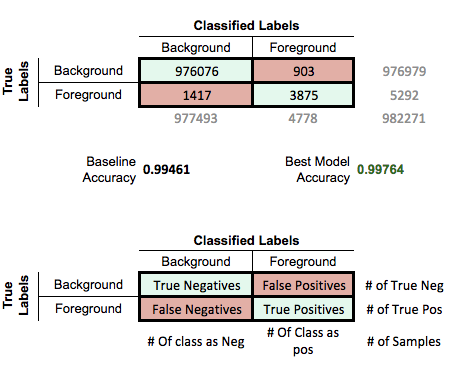
\includegraphics[width=0.3\linewidth]{confusionmatrix}
  \label{fig:confusionmatrix}
\end{figure}
\end{center}

The Confusion matrix \ref{fig:confusionmatrix} shows comparison between proposed baseline and best model accuracy. As it can be observed by the bold numbers in black and green, for the current testing set (the entire image 2 sample data), our model beats the baseline.

\begin{table}[h!]
\centering
 \begin{tabular}{||c c c||} 
 \hline
Model & Run time (mins) & Accuracy \\ [0.5ex] 
 \hline\hline
Random Forest & 22.8  & .99767   \\[1ex] 
 \hline
 SVM & 0  & 0 \\
\hline
KNN & 0  & 0 \\
\hline
 \end{tabular}
 \caption{Accuracy Comparison of Sequential vs. Parallel Environment}
 \label{tab:accuracy-comparison}
\end{table}


\section*{5 Conclusion}


\newpage

\begin{thebibliography}{9}

\bibitem{andrewng} 
Map-Reduce for Machine Learning on Multicore,
\\\texttt{http://www.andrewng.org/portfolio/map-reduce-for-machine-learning-on-multicore/}

\bibitem{amazonemr} 
Apache Spark - Amazon EMR,
\\\texttt{https://docs.aws.amazon.com/emr/latest/ReleaseGuide/emr-spark.html}

\bibitem{apachecheatsheet} 
Apache Spark Developer Cheat Sheet,
\\\texttt{https://mapr.com/ebooks/spark/apache-spark-cheat-sheet.html}

\bibitem{cross} 
Cross Validator Model,
\\\texttt{https://jaceklaskowski.gitbooks.io/mastering-apache-spark/content/spark-mllib/spark-mllib-CrossValidator.html}

\bibitem{compare} 
Classifier Comparison,
\\\texttt{http://scikit-learn.org/stable/auto\_examples/classification/plot\_classifier\_comparison.html}

\bibitem{ensembles} 
Classification by using Ensembles of Classifiers,
\\\texttt{https://grzegorzgajda.gitbooks.io/spark-examples/content/classification/rf-classification.html}


\bibitem{mllib} 
MLlib: Scalable Machine Learning on Spark
\\\texttt{https://web.stanford.edu/~rezab/sparkworkshop/slides/xiangrui.pdf}


\bibitem{ensemblesrdd} 
Ensembles - RDD-based API
\\\texttt{https://spark.apache.org/docs/latest/mllib-ensembles.html}

\bibitem{steps} 
EMR Add Steps
\\\texttt{https://docs.aws.amazon.com/cli/latest/reference/emr/add-steps.html}

\bibitem{decisiontree} 
Decision Tree
\\\texttt{https://spark.apache.org/docs/2.2.0/mllib-decision-tree.html}

\bibitem{randomforestclassifier} 
Random Forest Classifier
\\\texttt{http://scikit-learn.org/stable/modules/generated/sklearn.ensemble.RandomForestClassifier.html}

\bibitem{fft} 
Fast Fourier Transform
\\\texttt{https://en.m.wikipedia.org/wiki/Fast\_Fourier\_transform}

\bibitem{spark} 
Spark
\\\texttt{http://spark.apache.org/}


\bibitem{Zaharia} Matei Zaharia. \textsl{An Architecture for Fast and General Data Processing on
Large Clusters}. Association for Computing Machinery., 2014

\bibitem{learningspark} Holden Karau, Andy Konwinski, Patrick Wendell, and Matei Zaharia. \textsl{Learning Spark: Lightning-Fast Big Data Analytics}. O'Reilly Media Inc., 2015

\bibitem{sparkinaction} Petar Zecevic and Marko Bonaci. \textsl{Spark in Action}. Manning
Publications., 2016

\bibitem{sparkprogramming} 
Spark Programming Guide
\\\texttt{http://spark.apache.org/docs/latest/programming-guide.html}

\end{thebibliography}

\newpage

\appendix
\section*{Appendices}

\section{Visualizing the Input}

\begin{figure}[!h]
  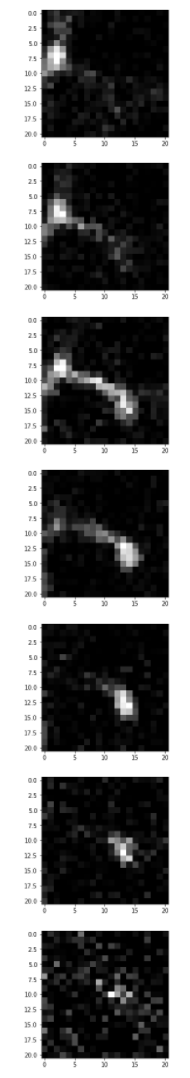
\includegraphics[width=0.15\linewidth]{neuron-slices}
  \label{fig:neuron-slices}
\end{figure}

\newpage

\section{Foreground And Background Analysis}
\begin{figure}[!h]
  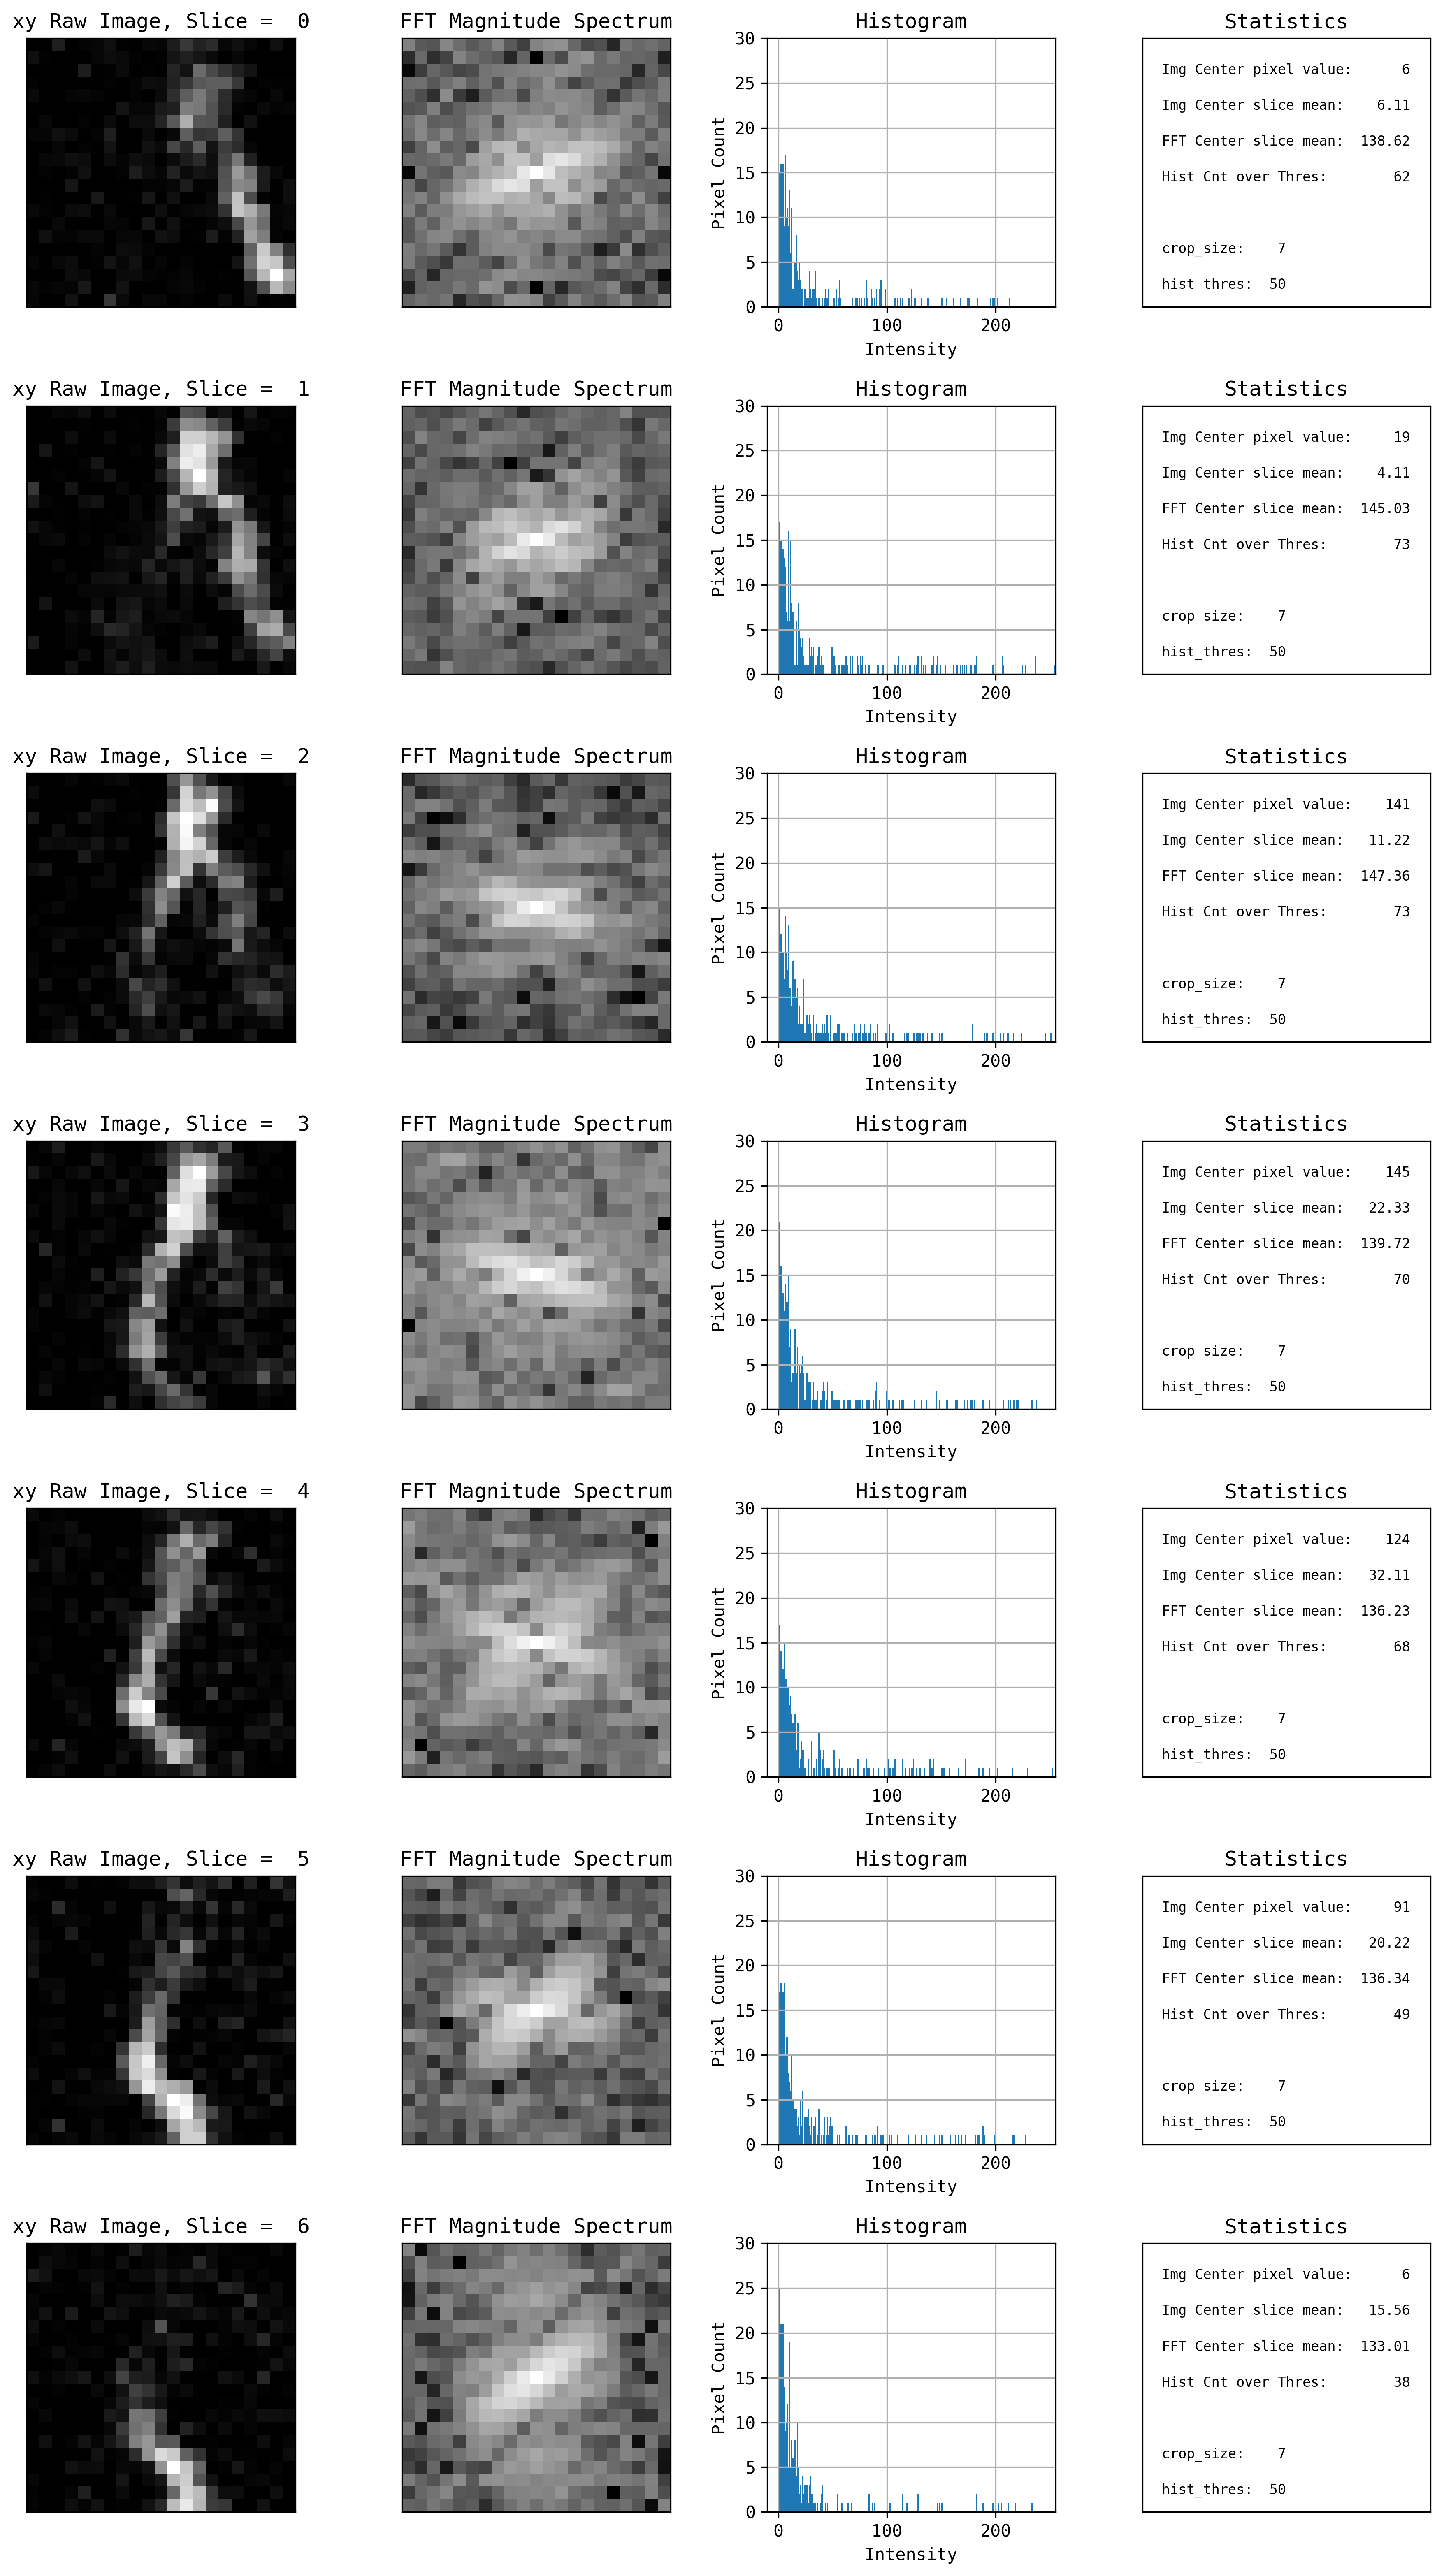
\includegraphics[width=0.5\linewidth]{foreground-xy-1}
  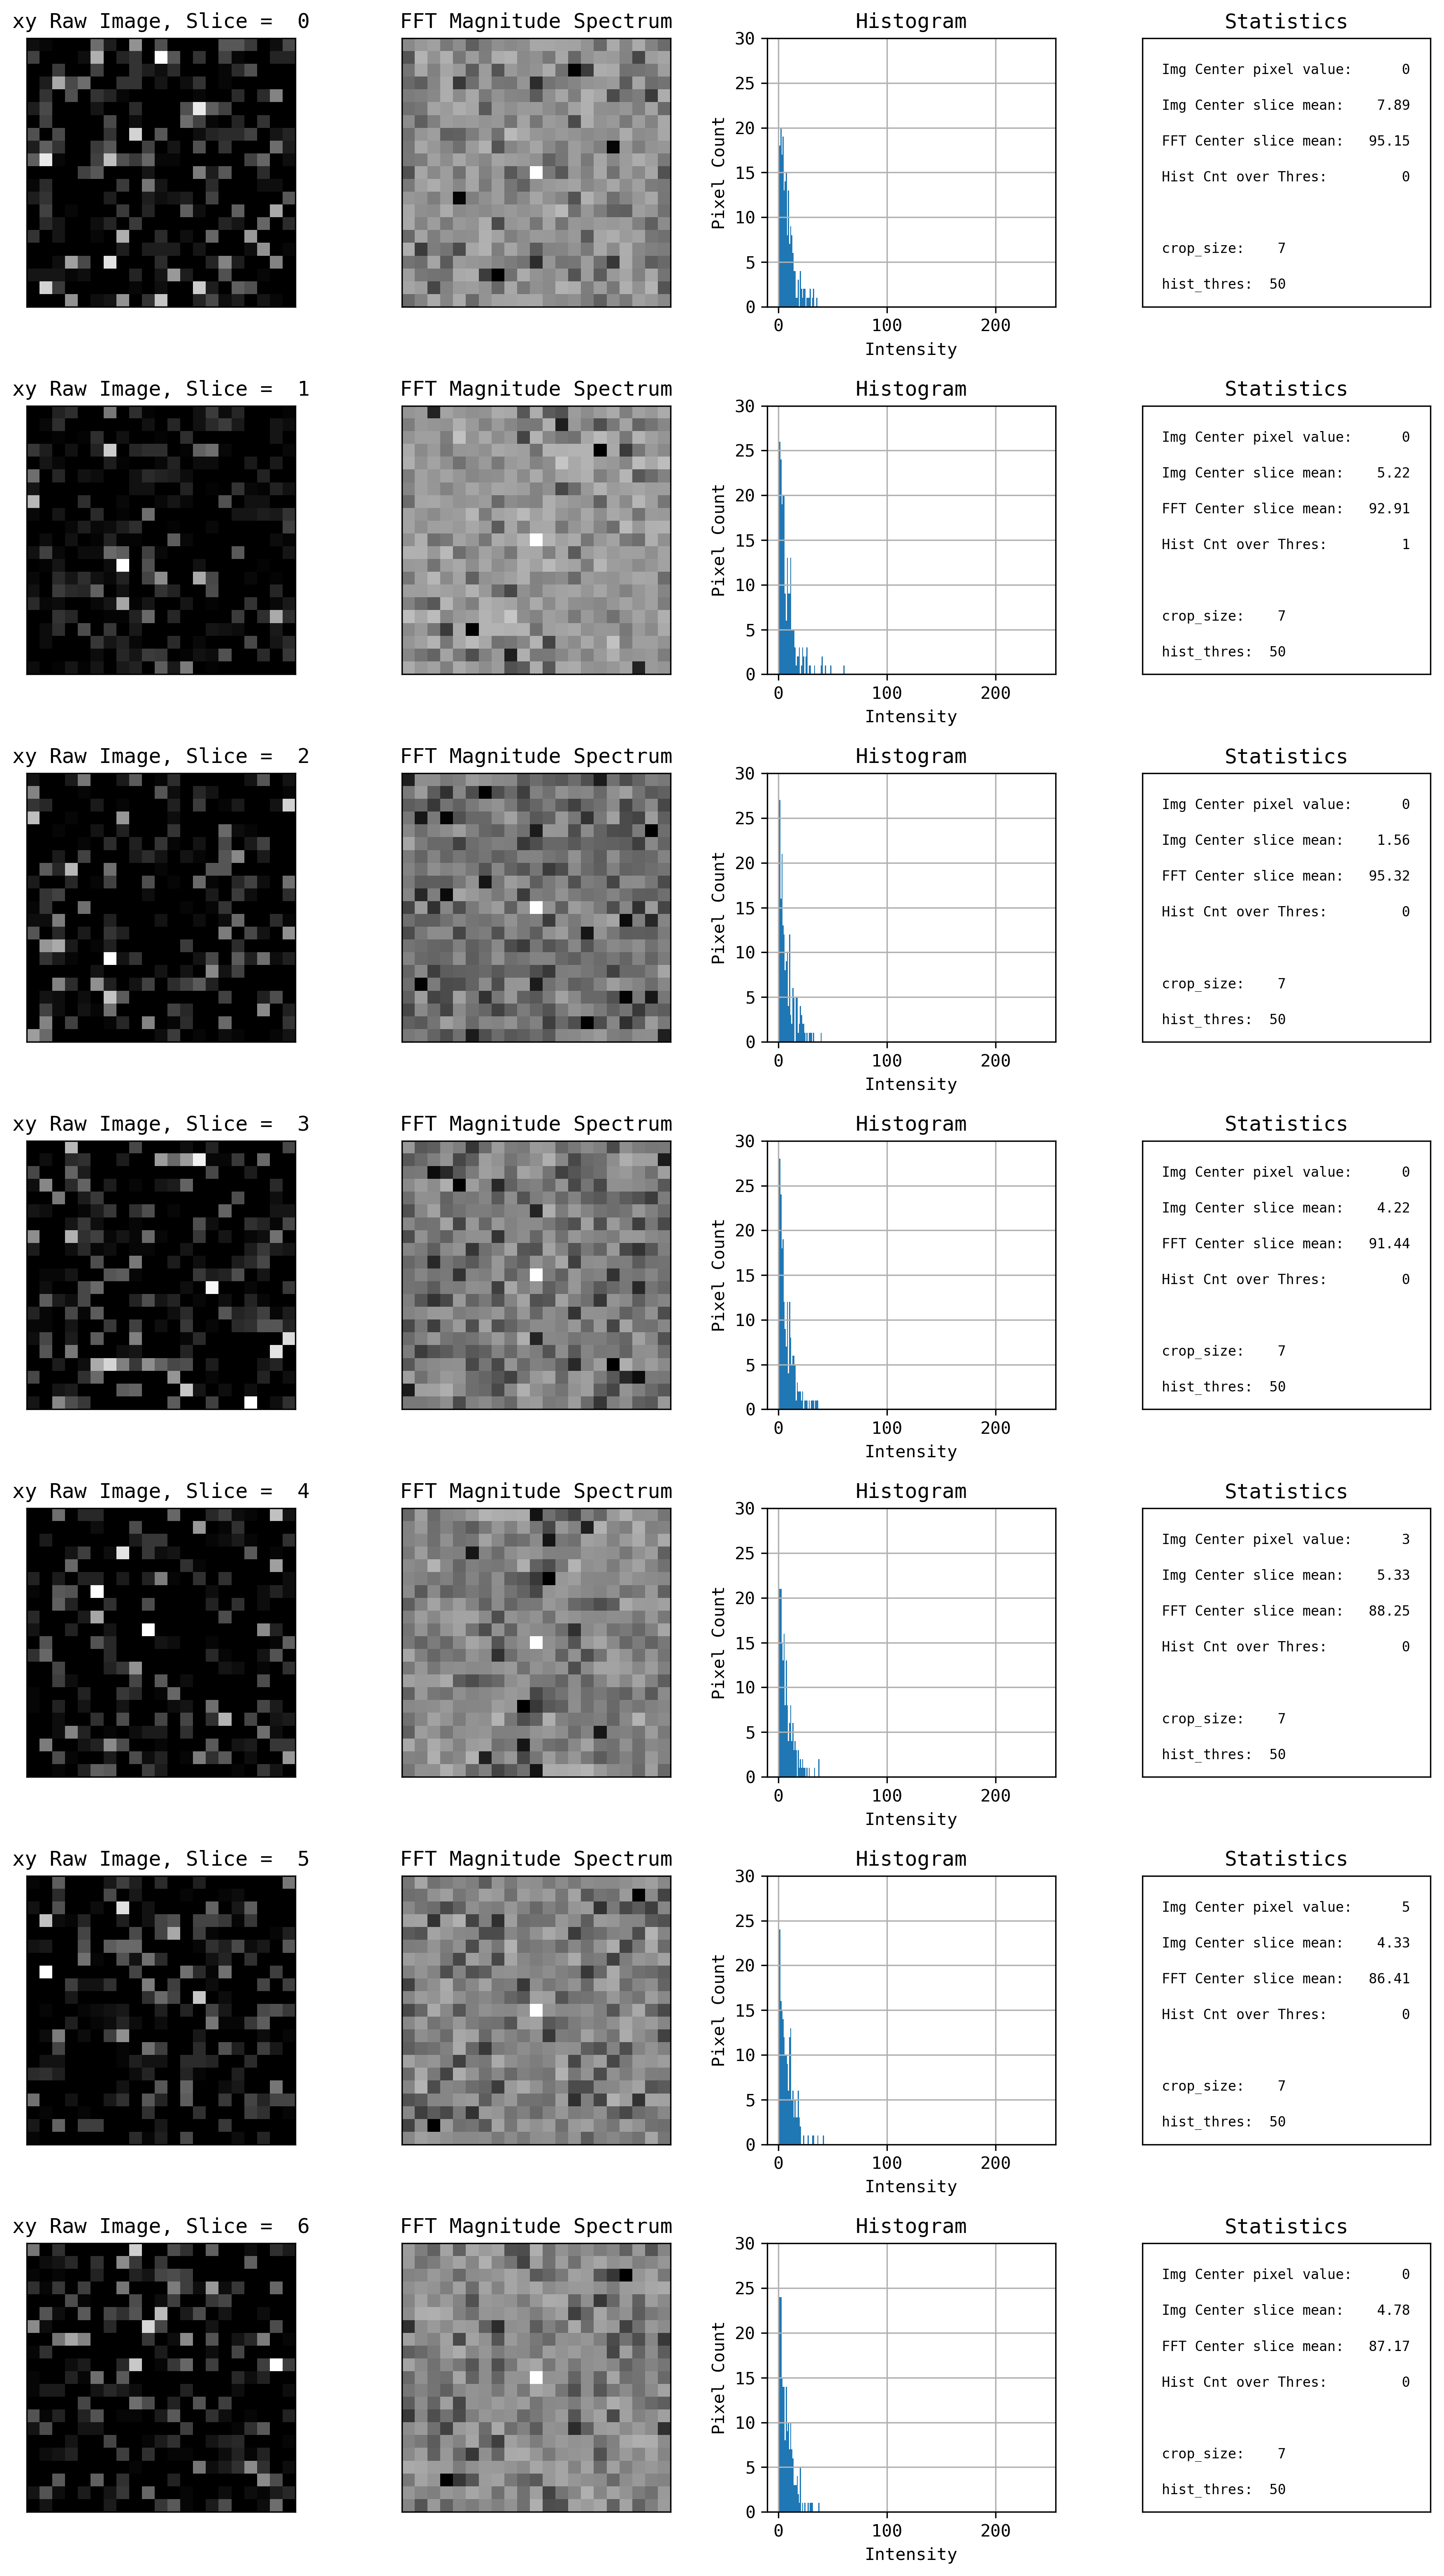
\includegraphics[width=0.5\linewidth]{background-xy-0}
  \label{fig:foreground-xy-1}
\end{figure}

\newpage

\section{Classification Comparison test}
\begin{figure}[!h]
  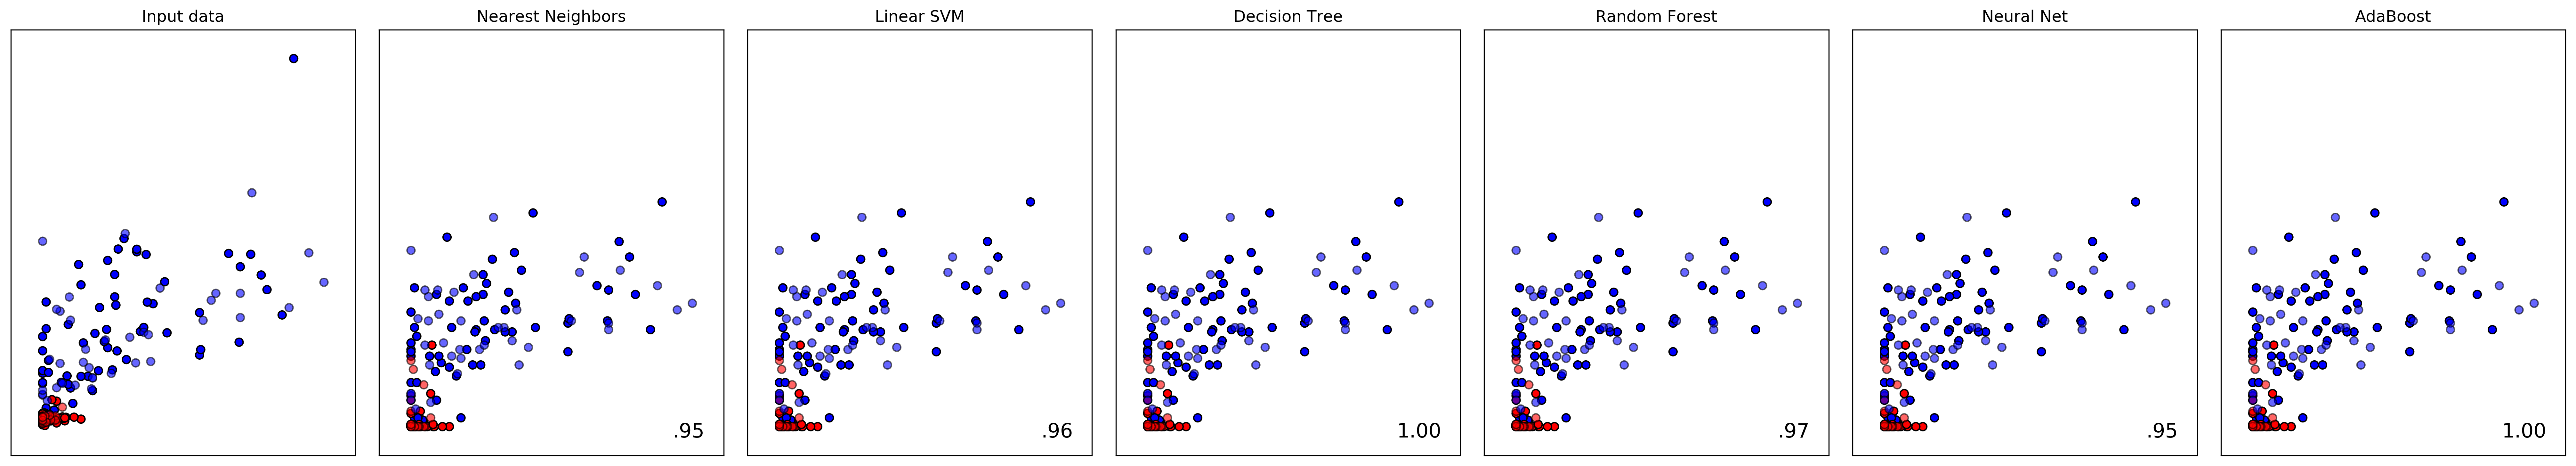
\includegraphics[width=1\linewidth]{classification-test}
  \label{fig:classification-test}
\end{figure}

\section{Application Pipeline}
\begin{figure}[!h]
  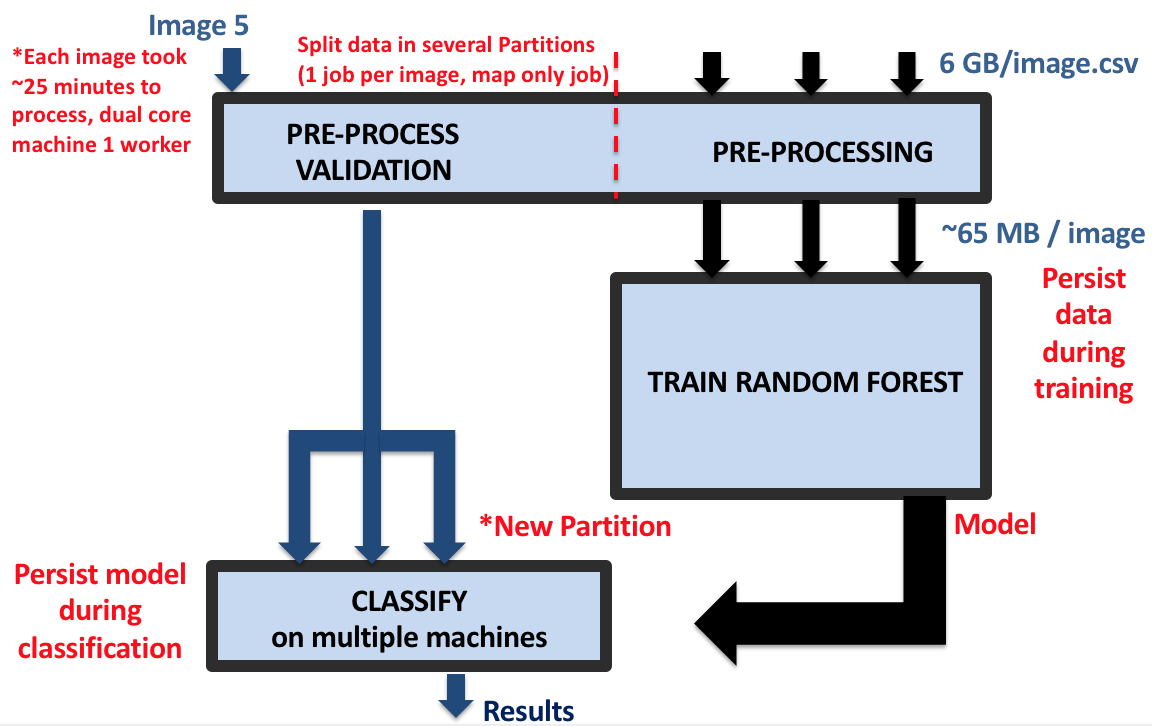
\includegraphics[width=0.7\linewidth]{pipeline}
  \label{fig:pipeline}
\end{figure}




\end{document}
